\section{Integration Techniques}

%%%%%%%%%%%%%%%%%%%%%%%%%%%%%%%%%%%%%
%  Fundamental Theorem of Calculus  %
%%%%%%%%%%%%%%%%%%%%%%%%%%%%%%%%%%%%%

\subsection{Fundamental Theorem of Calculus}

\Theorem{Fundamental Theorem of Calculus}{
    Let $f$ be a function defined on an open interval $I$ that contains $a$. If $f$ is continuous on $I$, then the function $F$ defined by
    \[
        F(x) = \int_a^x f(t) \dd{t}
    \]
    is uniformly continuous on $I$, differentiable on the open interval, and
    \[
        F'(x) = f(x)
    \]
    for all $x$ in the open interval.
}

%%%%%%%%%%%%%%%%%%%%%
%  Common Formulae  %
%%%%%%%%%%%%%%%%%%%%%

\subsection{Common Differentiation and Integration Formulae}

\begin{table}[H]
    \centering
    \begin{tabular}{l | l}
        \textbf{Derivative} & \textbf{Integral} \\
        \hline

        $\dv{}{x} x = 1$ , \quad $\dv{}{x} c = 0 $ & $\int c \dd{x} = cx + c$ \\
        $\dv{}{x} x^n $ & $\int x^n \dd{x} = \frac{x^{n+1}}{n+1} + c$ \\
        $\dv{}{x} \ln(x) = \frac{1}{x}$ & $\int \frac{1}{x} \dd{x} = \ln|x| + c$ \\ 
        $\dv{}{x} e^{mx} = me^{mx} $ & $\int e^{mx} \dd{x} = \frac{1}{m} e^{mx} + c$ \\
        $\dv{}{x} a^x = a^x \ln(a)$ & $\int a^x \dd{x} = \frac{1}{\ln(a)} a^x + c$ \\
        $\dv{}{x} \sin(mx) = m \cos(mx) $ & $\int \cos(mx) \dd{x} = \frac{1}{m} \sin(mx) + c$ \\
        $\dv{}{x} \cos(mx) = -m \sin(mx) $ & $\int \sin(mx) \dd{x} = -\frac{1}{m} \cos(mx) + c$ \\
        $\dv{}{x} \tan(x) = \sec^2(x)$ & $\int \sec^2(x) \dd{x} = \tan(x) + c$ \\
        $\dv{}{x} \cot(x) = -\csc^2(x)$ & $\int \csc^2(x) \dd{x} = -\cot(x) + c$ \\
        $\dv{}{x} \sec(x) = \sec(x) \tan(x)$ & $\int \sec(x) \tan(x) \dd{x} = \sec(x) + c$ \\
        $\dv{}{x} \csc(x) = -\csc(x) \cot(x)$ & $\int \csc(x) \cot(x) \dd{x} = -\csc(x) + c$ \\
        $\dv{}{x} \sin^{-1}(x) = \frac{1}{\sqrt{1-x^2}}$ & $\int \frac{1}{\sqrt{1-x^2}} \dd{x} = \sin^{-1}(x) + c$ \\
        $\dv{}{x} \cos^{-1}(x) = -\frac{1}{\sqrt{1-x^2}}$ & $\int \frac{1}{\sqrt{1-x^2}} \dd{x} = -\cos^{-1}(x) + c$ \\
        $\dv{}{x} \tan^{-1}(x) = \frac{1}{1+x^2}$ & $\int \frac{1}{1+x^2} \dd{x} = \tan^{-1}(x) + c$ \\
        $\dv{}{x} \cot^{-1}(x) = -\frac{1}{1+x^2}$ & $\int \frac{1}{1+x^2} \dd{x} = -\cot^{-1}(x) + c$ \\
        $\dv{}{x} \sec^{-1}(x) = \frac{1}{x \sqrt{x^2-1}}$ & $\int \frac{1}{x \sqrt{x^2-1}} \dd{x} = \sec^{-1}(x) + c$ \\
        $\dv{}{x} \csc^{-1}(x) = -\frac{1}{x \sqrt{x^2-1}}$ & $\int \frac{1}{x \sqrt{x^2-1}} \dd{x} = -\csc^{-1}(x) + c$ \\
        $\dv{}{x} \sqrt{x} = \frac{1}{2 \sqrt{x}}$ & $\int \frac{1}{\sqrt{x}} \dd{x} = 2\sqrt{x} + c$ \\
    \end{tabular}
    \caption{Common Differentiation and Integration Formulae}
\end{table}


%%%%%%%%%%%%%%%%%%%
%  More Formulae  %
%%%%%%%%%%%%%%%%%%%

\subsection{More Formulae}
\begin{enumerate}
    \begin{minipage}{0.5\textwidth}
        \item $\int \tan(x) \dd{x} = \ln\lvert \sec(x) \rvert + c$
    \end{minipage}
    \begin{minipage}{0.5\textwidth}
        \item $\int \csc(x) \dd{x} = \ln\lvert \tan\frac{x}{2} \rvert + c$
    \end{minipage} \\~\\
    \begin{minipage}{0.5\textwidth}
        \item $\int \sec(x) \dd{x} = \ln\lvert \sec(x) + \tan(x) \rvert + c$
    \end{minipage}
    \begin{minipage}{0.5\textwidth}
        \item $\int \sec(x) \dd{x} = \ln\lvert \tan(\frac{\pi}{4} + \frac{x}{2}) \rvert$
    \end{minipage}
        \item $\int \csc(x) \dd{x} = -\ln\lvert \csc(x) + \cot(x) \rvert + c$
        \item $\int \frac{1}{a^2+x^2} \dd{x} = \frac{1}{a} \tan^{-1}(\frac{x}{a}) + c$ \\~\\
    \begin{minipage}{0.5\textwidth}
        \item $\int \frac{1}{a^2-x^2} \dd{x} = \frac{1}{2a} \ln\lvert \frac{a+x}{a-x} \rvert + c$
    \end{minipage}
    \begin{minipage}{0.5\textwidth}
        \item $\int \frac{1}{x^2-a^2} \dd{x} = \frac{1}{2a} \ln\lvert \frac{a-x}{a+x} \rvert + c$
    \end{minipage} \\~\\
    \begin{minipage}{0.5\textwidth}
        \item $\int \frac{1}{\sqrt{x^2+a^2}} \dd{x} = \ln\lvert x + \sqrt{x^2+a^2} \rvert + c$
    \end{minipage}
    \begin{minipage}{0.5\textwidth}
        \item $\int \frac{1}{\sqrt{a^2-x^2}} \dd{x} = \sin^{-1}(\frac{x}{a}) + c$
    \end{minipage}
    \item $\int \sqrt{a^2 - x^2} \dd{x} = \frac{x \sqrt{a^2-x^2}}{2} + \frac{a^2}{2} \sin^{-1} \frac{x}{a} + c$
    \item $\int e^x \left[ f(x) + f'(x) \right] \dd{x} = e^x f(x) + c$
\end{enumerate}


%%%%%%%%%%%%%%%%%%%%%%%%%%
%  Integration by Parts  %
%%%%%%%%%%%%%%%%%%%%%%%%%%

\subsection{Integration by Parts}

\Theorem{Integration by Parts}{
    Let $u$ and $v$ be differentiable functions of $x$. Then,
    \[
        \int uv \dd{x} = u \int v \dd{x} - \int \left[ \dv{u}{x} \int v \dd{x} \right] \dd{x}
    \]
    Or,
    \[ 
       \int u \dd{v} = uv - \int v \dd{u}
   \]
}

\underline{\textbf{Proof:}} \\ 
Let $u = u(x)$ and $w = w(x)$. Then,
\[
    \dv{(uw)}{x} = u \dv{w}{x} + w \dv{u}{x}
\]
Integrating both sides, we get
\[
    \int \dv{(uw)}{x} \dd{x} = \int u \dv{w}{x} \dd{x} + \int w \dv{u}{x} \dd{x}
\]
Or,
\[
    uw = \int u \dv{w}{x} \dd{x} + \int w \dv{u}{x} \dd{x}
\]
Rearranging, we get
\[
    \int u \dv{w}{x} \dd{x} = uw + c - \int w \dv{u}{x} \dd{x}
\]
Let $v = \dv{w}{x}$, then $w = \int v \dd{x}$. Hence,
\[
    \int uv \dd{x} = u \int v \dd{x} - \int \left[ \dv{u}{x} \int v \dd{x} \right] \dd{x}
\]
\qed


%%%%%%%%%%%%%%%%%%%%%%%%%%%%
%  Method of Substitution  %
%%%%%%%%%%%%%%%%%%%%%%%%%%%%

\subsection{Method of Substitution}
\begin{enumerate}[label=\Alph*.]
    \item $\int \frac{1}{(ax+b)\sqrt{cx+d}} \dd{x}$ \quad Let $cx+d = z^2$
    \item $\int \frac{1}{\sin^m x \cos^m x} \dd{x}$ \quad If $m+n = p$ is even, multiply and divide by $\sec^p x$ and let $\tan x = z$.
    \item $\int \frac{1}{\sin^m x + \cos^m x} \dd{x}$ \quad If $m$ is even, mulpliply and divide by $\sec^m x$.
    \item $\int \frac{\cos x}{a \cos x + b \sin x} \dd{x}$ \quad Write $nom = l \times (denom) + m \times (denom)'$, then determine $l$ and $m$.
    \item $\int \frac{\cos x}{a \cos x + b \sin x} \dd{x} + c$ \quad Write $\sin x$ and $\cos x$ as $\tan \frac{x}{2}$.
    \item $\int \frac{1}{\sqrt{x^2 + a^2}} \dd{x}$ \quad Let $x = a \tan \theta$
    \item $\int \frac{1}{\sqrt{x^2 - a^2}} \dd{x}$ \quad Let $x = a \sec \theta$
    \item $\int \sqrt{a^2 - x^2} \dd{x}$ \quad Let $x = a \sin \theta$
\end{enumerate}


%%%%%%%%%%%%%%%%%%%%%%%%%%%%%
%  Trigonometric Integrals  %
%%%%%%%%%%%%%%%%%%%%%%%%%%%%%

\subsection{Trigonometric Integrals}

\begin{table}[htpb]
    \centering
    \begin{tabular}{c | c | c | c}
        \textbf{Form} & \textbf{Looks like} & \textbf{Substitution} & \textbf{Limit Assumption} \\
        \hline
        $\sqrt{b^2x^2 - a^2}$ & $\sec^{2}\theta - 1 = \tan^{2}\theta$ & $x = \frac{a}{b} \sec\theta$ & $0 \leq \theta < \frac{\pi}{2}, \frac{\pi}{2} < \theta \leq \pi$ \\ 
        $\sqrt{a^2 - b^2x^2}$ & $1 - \sin^{2}\theta = \cos^{2}\theta$ & $x = \frac{a}{b} \sin\theta$ & $-\frac{\pi}{2} \leq \theta \leq \frac{\pi}{2}$ \\
        $\sqrt{a^2 + b^2x^2}$ & $\tan^{2}\theta + 1 = \sec^{2}\theta$ & $x = \frac{a}{b} \tan\theta$ & $-\frac{\pi}{2} < \theta < \frac{\pi}{2}$ \\
    \end{tabular}
    \caption{Trigonometric Integral Substitution}
\end{table}


%%%%%%%%%%%%%%%%%%%%%%%
%  Partial Fractions  %
%%%%%%%%%%%%%%%%%%%%%%%

\subsection{Partial Fractions}

\begin{table}[htpb]
    \centering
    \begin{tabular}{c | c}
        \textbf{Factor in denominator} & \textbf{Term in partial fraction decomposition} \\ 
        \hline 
        $ax + b$ & $\frac{A}{ax + b}$ \\ 
        $(ax + b)^k$ & $\frac{A_1}{ax+b} + \frac{A_2}{(ax+b)^2} + \dots + \frac{A_k}{(ax+b)^k}$ \\ 
        $ax^2 + bx + c$ & $\frac{Ax + b}{ax^2 + bx + c}$ \\ 
        $(ax^2 + bx + c)^k$ & $\frac{A_1x + B_1}{ax^2+bx+c} + \frac{A_2x + B_2}{(ax^2+bx+c)^2} + \dots + \frac{A_kx + B_k}{(ax^2+bx+c)^k}$ \\
    \end{tabular}
    \caption{Partial Fraction Decomposition}
\end{table}


%%%%%%%%%%%%%%%%%%%%%%%%%%%%%%%%%%%
%  Integrals Involving Roots      %
%%%%%%%%%%%%%%%%%%%%%%%%%%%%%%%%%%%

\subsection{Integrals Involving Roots}

For integrals involving $\sqrt{a^2 - x^2}$, $\sqrt{a^2 + x^2}$, or $\sqrt{x^2 - a^2}$, use trigonometric substitution:

\begin{table}[htpb]
    \centering
    \begin{tabular}{c | c | c}
        \textbf{Expression} & \textbf{Substitution} & \textbf{Identity Used} \\ 
        \hline 
        $\sqrt{a^2 - x^2}$ & $x = a\sin\theta$ & $1 - \sin^2\theta = \cos^2\theta$ \\ 
        $\sqrt{a^2 + x^2}$ & $x = a\tan\theta$ & $1 + \tan^2\theta = \sec^2\theta$ \\ 
        $\sqrt{x^2 - a^2}$ & $x = a\sec\theta$ & $\sec^2\theta - 1 = \tan^2\theta$ \\
    \end{tabular}
    \caption{Trigonometric Substitutions for Roots}
\end{table}

\begin{center}
\textbf{Reference Triangles for Trigonometric Substitution}

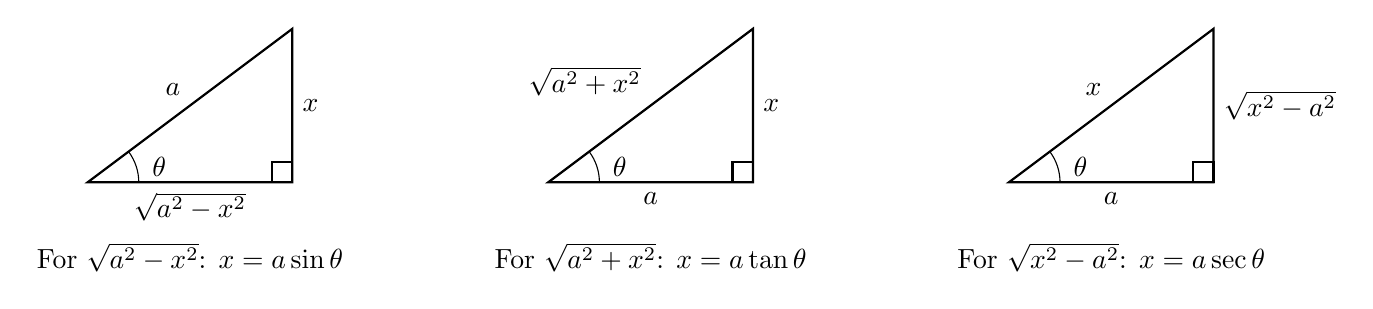
\begin{tikzpicture}[scale=1.3]
    % Triangle 1: x = a*sin(theta), for sqrt(a^2 - x^2)
    \draw[thick] (0,0) -- (2,0) node[midway, below] {$\sqrt{a^2-x^2}$} -- (2,1.5) node[midway, right] {$x$} -- cycle;
    \draw[thick] (2,0) rectangle (1.8,0.2);
    \draw (0.5,0) arc (0:36.87:0.5);
    \node at (0.7,0.15) {$\theta$};
    \node[above left] at (1,0.75) {$a$};
    \node[below] at (1,-0.5) {For $\sqrt{a^2-x^2}$: $x = a\sin\theta$};
    
    % Triangle 2: x = a*tan(theta), for sqrt(a^2 + x^2)
    \begin{scope}[xshift=4.5cm]
        \draw[thick] (0,0) -- (2,0) node[midway, below] {$a$} -- (2,1.5) node[midway, right] {$x$} -- cycle;
        \draw[thick] (2,0) rectangle (1.8,0.2);
        \draw (0.5,0) arc (0:36.87:0.5);
        \node at (0.7,0.15) {$\theta$};
        \node[above left] at (1,0.75) {$\sqrt{a^2+x^2}$};
        \node[below] at (1,-0.5) {For $\sqrt{a^2+x^2}$: $x = a\tan\theta$};
    \end{scope}
    
    % Triangle 3: x = a*sec(theta), for sqrt(x^2 - a^2)
    \begin{scope}[xshift=9cm]
        \draw[thick] (0,0) -- (2,0) node[midway, below] {$a$} -- (2,1.5) node[midway, right] {$\sqrt{x^2-a^2}$} -- cycle;
        \draw[thick] (2,0) rectangle (1.8,0.2);
        \draw (0.5,0) arc (0:36.87:0.5);
        \node at (0.7,0.15) {$\theta$};
        \node[above left] at (1,0.75) {$x$};
        \node[below] at (1,-0.5) {For $\sqrt{x^2-a^2}$: $x = a\sec\theta$};
    \end{scope}
\end{tikzpicture}
\end{center}

\Example{Evaluate $\int \frac{1}{\sqrt{9-x^2}} \dd{x}$}
{
    Here $a=3$, so let $x = 3\sin\theta$, thus $\dd{x} = 3\cos\theta \dd{\theta}$.
    \begin{align*}
        \int \frac{1}{\sqrt{9-x^2}} \dd{x} &= \int \frac{3\cos\theta}{\sqrt{9-9\sin^2\theta}} \dd{\theta} \\
        &= \int \frac{3\cos\theta}{3\cos\theta} \dd{\theta} \\
        &= \int 1 \dd{\theta} \\
        &= \theta + c \\
        &= \sin^{-1}\left(\frac{x}{3}\right) + c
    \end{align*}
}


%%%%%%%%%%%%%%%%%%%%%%%%%%%%%%%%%%%
%  Integrals Involving Quadratics %
%%%%%%%%%%%%%%%%%%%%%%%%%%%%%%%%%%%

\subsection{Integrals Involving Quadratics}

For integrals involving $ax^2 + bx + c$, complete the square first:
\[ ax^2 + bx + c = a\left[\left(x + \frac{b}{2a}\right)^2 + \frac{4ac - b^2}{4a^2}\right] \]

Then use substitution $u = x + \frac{b}{2a}$ to convert to standard forms.

\Example{Evaluate $\int \frac{1}{x^2 + 4x + 13} \dd{x}$}{
    Complete the square:
    \[ x^2 + 4x + 13 = (x+2)^2 + 9 = (x+2)^2 + 3^2 \]
    Let $u = x+2$, so $\dd{u} = \dd{x}$:
    \begin{align*}
        \int \frac{1}{x^2 + 4x + 13} \dd{x} &= \int \frac{1}{u^2 + 9} \dd{u} \\
        &= \frac{1}{3}\tan^{-1}\left(\frac{u}{3}\right) + c \\
        &= \frac{1}{3}\tan^{-1}\left(\frac{x+2}{3}\right) + c
    \end{align*}
}


%%%%%%%%%%%%%%%%%%%%%%%%%%%%%%%%%%%
%  Integration Strategy           %
%%%%%%%%%%%%%%%%%%%%%%%%%%%%%%%%%%%

\subsection{Integration Strategy}

When faced with an integral, use the following strategy:

\begin{enumerate}
    \item \textbf{Simplify the integrand}: Expand, factor, or use algebraic manipulation
    \item \textbf{Look for obvious substitutions}: If $u' = g'(x)$ appears, try $u = g(x)$
    \item \textbf{Classify by type}:
        \begin{itemize}
            \item Trigonometric integrals $\to$ use trig identities
            \item Rational functions $\to$ use partial fractions
            \item Products $\to$ try integration by parts
            \item Roots of quadratics $\to$ complete the square or trig substitution
        \end{itemize}
    \item \textbf{Try different techniques}: If one method fails, try another
    \item \textbf{Use tables or computer algebra systems}: For complex integrals
\end{enumerate}


%%%%%%%%%%%%%%%%%%%%%%%%%%%%%%%%%%%%%%%%%%%
%  Approximating Definite Integrals      %
%%%%%%%%%%%%%%%%%%%%%%%%%%%%%%%%%%%%%%%%%%%

\subsection{Approximating Definite Integrals}

When an antiderivative cannot be found in closed form, use numerical approximation methods.

\subsubsection{Midpoint Rule}

Divide $[a,b]$ into $n$ subintervals of width $\Delta x = \frac{b-a}{n}$. Let $\bar{x}_i$ be the midpoint of the $i$-th subinterval.
\[ \int_{a}^{b} f(x) \dd{x} \approx M_n = \Delta x \sum_{i=1}^{n} f(\bar{x}_i) \]

\subsubsection{Trapezoidal Rule}

\[ \int_{a}^{b} f(x) \dd{x} \approx T_n = \frac{\Delta x}{2} \left[f(x_0) + 2f(x_1) + 2f(x_2) + \dots + 2f(x_{n-1}) + f(x_n)\right] \]

\subsubsection{Simpson's Rule}

Requires $n$ to be even. Approximates the function with parabolas instead of lines:
\[ \int_{a}^{b} f(x) \dd{x} \approx S_n = \frac{\Delta x}{3} \left[f(x_0) + 4f(x_1) + 2f(x_2) + 4f(x_3) + \dots + 2f(x_{n-2}) + 4f(x_{n-1}) + f(x_n)\right] \]

\Note{
    Simpson's Rule is generally more accurate than the Trapezoidal Rule, which is more accurate than the Midpoint Rule for the same number of subintervals.
}

\begin{center}
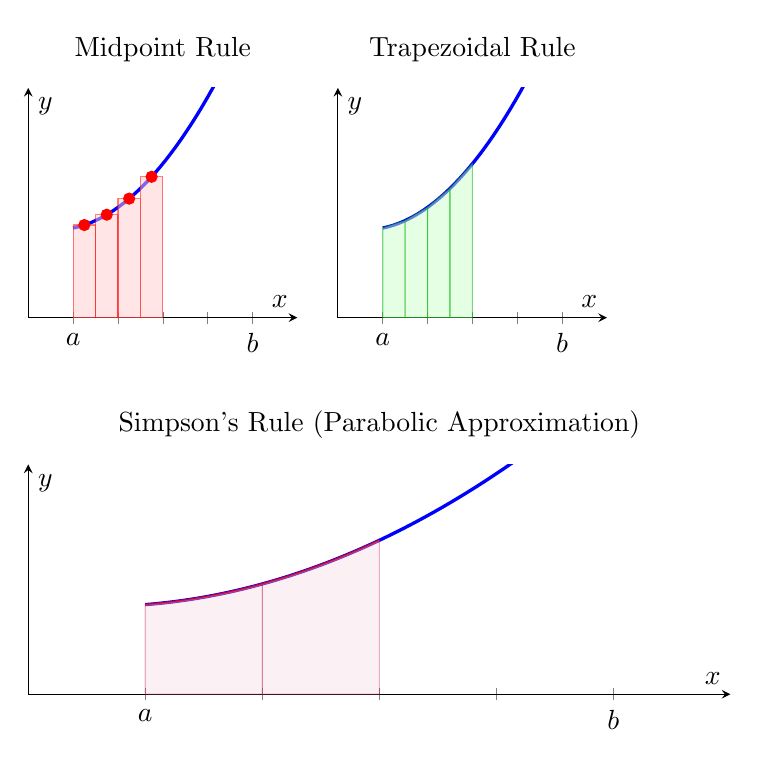
\begin{tikzpicture}
    % Midpoint Rule
    \begin{axis}[
        name=midpoint,
        width=5cm, height=4.5cm,
        axis lines=center,
        xlabel=$x$, ylabel=$y$,
        xmin=0, xmax=3,
        ymin=0, ymax=2.5,
        domain=0.5:2.5,
        samples=50,
        title={Midpoint Rule},
        ytick=\empty,
        xtick={0.5,1,1.5,2,2.5},
        xticklabels={$a$,,,,$b$},
        ]
        % The function
        \addplot[blue, very thick] {0.5*x^2 - 0.3*x + 1};
        
        % Rectangles (n=4)
        \addplot[red, fill=red!20, opacity=0.5] coordinates {(0.5,1.00781) (0.75,1.00781) (0.75,0) (0.5,0)} -- cycle;
        \addplot[red, fill=red!20, opacity=0.5] coordinates {(0.75,1.12031) (1,1.12031) (1,0) (0.75,0)} -- cycle;
        \addplot[red, fill=red!20, opacity=0.5] coordinates {(1,1.29531) (1.25,1.29531) (1.25,0) (1,0)} -- cycle;
        \addplot[red, fill=red!20, opacity=0.5] coordinates {(1.25,1.53281) (1.5,1.53281) (1.5,0) (1.25,0)} -- cycle;
        
        % Midpoints
        \addplot[red, only marks, mark=*, mark size=2pt] coordinates {(0.625,1.00781) (0.875,1.12031) (1.125,1.29531) (1.375,1.53281)};
    \end{axis}
    
    % Trapezoidal Rule
    \begin{axis}[
        at={(midpoint.right of south east)}, anchor=left of south west,
        xshift=0.5cm,
        width=5cm, height=4.5cm,
        axis lines=center,
        xlabel=$x$, ylabel=$y$,
        xmin=0, xmax=3,
        ymin=0, ymax=2.5,
        domain=0.5:2.5,
        samples=50,
        title={Trapezoidal Rule},
        ytick=\empty,
        xtick={0.5,1,1.5,2,2.5},
        xticklabels={$a$,,,,$b$},
        ]
        % The function
        \addplot[blue, very thick] {0.5*x^2 - 0.3*x + 1};
        
        % Trapezoids (n=4)
        \addplot[green!70!black, fill=green!20, opacity=0.5] coordinates {(0.5,0.975) (0.75,1.05625) (0.75,0) (0.5,0)} -- cycle;
        \addplot[green!70!black, fill=green!20, opacity=0.5] coordinates {(0.75,1.05625) (1,1.2) (1,0) (0.75,0)} -- cycle;
        \addplot[green!70!black, fill=green!20, opacity=0.5] coordinates {(1,1.2) (1.25,1.40625) (1.25,0) (1,0)} -- cycle;
        \addplot[green!70!black, fill=green!20, opacity=0.5] coordinates {(1.25,1.40625) (1.5,1.675) (1.5,0) (1.25,0)} -- cycle;
    \end{axis}
    
    % Simpson's Rule
    \begin{axis}[
        at={(midpoint.below south west)}, anchor=above north west,
        yshift=-0.5cm,
        width=10.5cm, height=4.5cm,
        axis lines=center,
        xlabel=$x$, ylabel=$y$,
        xmin=0, xmax=3,
        ymin=0, ymax=2.5,
        domain=0.5:2.5,
        samples=100,
        title={Simpson's Rule (Parabolic Approximation)},
        ytick=\empty,
        xtick={0.5,1,1.5,2,2.5},
        xticklabels={$a$,,,,$b$},
        ]
        % The function
        \addplot[blue, very thick] {0.5*x^2 - 0.3*x + 1};
        
        % Parabolic segments (n=4)
        \addplot[purple, thick, domain=0.5:1] {0.5*x^2 - 0.3*x + 1};
        \addplot[purple, fill=purple!20, opacity=0.3, domain=0.5:1] {0.5*x^2 - 0.3*x + 1} \closedcycle;
        
        \addplot[purple, thick, domain=1:1.5] {0.5*x^2 - 0.3*x + 1};
        \addplot[purple, fill=purple!20, opacity=0.3, domain=1:1.5] {0.5*x^2 - 0.3*x + 1} \closedcycle;
    \end{axis}
\end{tikzpicture}
\captionof{figure}{Comparison of Numerical Integration Methods for $\int_a^b f(x) \dd{x}$}
\end{center}


%%%%%%%%%%%%%%%%%%%%%%%%
%  Improper Integrals  %
%%%%%%%%%%%%%%%%%%%%%%%%

\subsection{Improper Integrals}

\Definition{Improper Integrals}{
    An integral is said to be \textbf{improper} if one of the following conditions is met:
    \begin{enumerate}
        \item The interval of integration is infinite.
        \item The integrand is discontinuous at one or more points in the interval of integration. 
    \end{enumerate}
    The integral is said to \textbf{converge} if the limit of the integral exists, and \textbf{diverge} otherwise.
}

\begin{enumerate}[label=\textbf{Type-\arabic*:}, leftmargin=*, align=left]
    \item If $\int_{a}^{t} f(x) \dd{x}$ exists for all $t>a$, then \[ 
        \int_{a}^{\infty} f(x) \dd{x} = \lim_{t \to \infty} \int_{a}^{t} f(x) \dd{x}
    \] provided the limit exists and is finite.
    \item If $\int_{t}^{b} f(x) \dd{x}$ exists for all $t<b$, then \[ 
        \int_{-\infty}^{b} f(x) \dd{x} = \lim_{t \to -\infty} \int_{t}^{b} f(x) \dd{x}
    \] provided the limit exists and is finite.
    \item If $\int_{-\infty}^{c} f(x) \dd{x}$ and $\int_{c}^{\infty} f(x) \dd{x}$ are both convergent, then \[ 
        \int_{-\infty}^{\infty} f(x) \dd{x} = \int_{-\infty}^{c} f(x) \dd{x} + \int_{c}^{\infty} f(x) \dd{x}
    \]
    \item $\int_a^b f(x) \dd{x}$ \quad If $f(x)$ is discontinuous at $x = c$, then \[
        \int_a^b f(x) \dd{x} = \lim_{\epsilon \to 0} \left[ \int_a^{c-\epsilon} f(x) \dd{x} + \int_{c+\epsilon}^b f(x) \dd{x} \right]
    \]
\end{enumerate}

\Note{
    If $a>0$ then \[ 
        \int_{a}^{\infty} \frac{1}{x^p} \dd{x}
    \] converges if $p>1$ and diverges if $p \leq 1$.
}

\subsubsection{Comparison Test}

\Theorem{Comparison Theorem}{
    If $f(x) \geq g(x) \geq 0$ on the interval $[a,\infty)$, then
    \begin{enumerate}
        \item If $\int_{a}^{\infty} f(x) \dd{x}$ converges, then so does $\int_{a}^{\infty} g(x) \dd{x}$.
        \item If $\int_{a}^{\infty} g(x) \dd{x}$ diverges, then so does $\int_{a}^{\infty} f(x) \dd{x}$.
    \end{enumerate}
}

\Example{Determine if the following integral is convergent or divergent: \[ 
    \int_{2}^{\infty} \frac{\cos^2x}{x^2} \dd{x}
\]}
{
    Notice that the numerator is bounded since \[
        0 \leq \cos^2x \leq 1
    \]Hence, it's likely that the denominator will determine the convergence of the integral. Since $p=2>1$, \[
        \int_{2}^{\infty} \frac{1}{x^2} \dd{x}
    \] is convergent. Since \[ 
        \frac{\cos^2x}{x^2} \leq \frac{1}{x^2}
    \] and $\int_{2}^{\infty} \frac{1}{x^2} \dd{x}$ is convergent, by the comparison test, \[
        \int_{2}^{\infty} \frac{\cos^2x}{x^2} \dd{x}
    \] is convergent.
}

\Example{Determine if the following integral is convergent or divergent: \[ 
    \int_{3}^{\infty} \frac{1}{x+e^{x}} \dd{x}
\]}
{
    In this case, the denominator determines the convergence of the integral. If we can find a larger function that converges, then the integral will converge. Notice that \[ 
        \frac{1}{x+e^{x}} < \frac{1}{e^{x}} = e^{-x}
    \]
    Also,
    \begin{align*}
        \int_{3}^{\infty} e^{-x} \dd{x} &= \lim_{t \to \infty} \int_{3}^{t} e^{-x} \dd{x} \\
                                        &= \lim_{t \to \infty} \left( -e^{-t} + e^{-3} \right) \\
                                        &= e^{-3}
    \end{align*}
    So, $\int_{3}^{\infty} e^{-x} \dd{x}$ is convergent. Therefore, by the Comparison test, \[ 
        \int_{3}^{\infty} \frac{1}{x+e^{x}} \dd{x}
    \] is also convergent.
}
